% testar algoritmos de seleção de características com instâncias reais
% tipo de instância: aprendizado de máquina
% função de custo utilizada
%   -> usamos a MCE
%   -> hipótese u-curve não vale
%   -> adequação dos dados as função de custo MCE
% como avaliar? Validando o modelo
% o modelo usado é o de support vector machine
%   -> C-SVC
%   -> kernel linear
%   -> C = 100
% validação cruzada:
%   -> 10-fold se +100 amostras
%   -> leave-one-out caso contrário
% datasets utilizados
% resultados dos experimentos



Com o objetivo de testar os algoritmos de seleção de características
em problemas reais, decidimos aplicá-los a problemas de seleção de 
modelos de aprendizado computacional. Usamos as características 
selecionadas para definir um modelo de aprendizado e calculamos o erro
de classificação médio para este modelo, usando validação cruzada. Os
dados utilizados estão disponíveis no 
\href{https://archive.ics.uci.edu/ml/index.php}{University of California Irvine (UCI) Machine Learning 
Repository}~\cite{Lic13}.

\section{Seleção de características em aprendizado de máquina}
Os dados disponíveis no repositório UCI Machine Learning Repository
são dados de treinamento e teste de aprendizado de máquina 
supervisionado. Estes dados são compostos por múltiplos exemplos de 
tuplas com valores de características do conjunto $S$ e o rótulo da 
tupla observada, $Y$. Um modelo de aprendizado determina um conjunto de 
possíveis classificadores para o problema; quando usamos seleção de 
características, indicando que um conjunto de características 
$X \in \powerset(S)$ descreve melhor os dados, estamos escolhendo como 
modelo de aprendizado o conjunto de classificadores que leva em 
consideração apenas as características de $X$.

Para que o conjunto $X$ de características selecionadas de fato 
determine um bom conjunto de classificadores, precisamos construir
o problema de seleção de características de maneira que isto aconteça.
Então, além de determinar que o conjunto de características seja $S$,
precisamos escolher a função de custo $c$ para o problema. 
Como discutido na seção~\ref{fund_concept:mce}, a função de custo
entropia condicional média (MCE), apresentada na equação~\ref{cost_function:mce}, faz bem este papel. Além disso, a 
função MCE induz curvas em U, com poucas violações, nas cadeias do 
reticulado Booleano. Por conta das violações, este problema não é o
U-Curve, porém, como visto no trabalho de Reis ~\cite{Rei12}, podemos 
aproximar a solução do problema original pela solução encontrada 
assumindo que estamos no caso U-Curve.

A função de custo MCE que utilizamos neste trabalho, disponível no
arcabouço \toolname{featsel}~\cite{Reis+17}, assume que os valores
das características são discretos, portanto ainda é necessário 
discretizar alguns dados de treinamento do UCI, que tiverem variáveis 
contínuas, para fazermos a seleção de características com o arcabouço.
A estratégia que utilizamos para tal tarefa é de 
discretizar os valores de características contínuas por quartis, 
mapeando seus valores para um inteiro entre 0 e 3. Existem entretanto 
outras estratégias mais elaboradas, como a de Fayyad e Irani~\cite{FI93}
que separa dados por classes minimizando uma medida de entropia média 
destas classes.

\section{Support Vector Machine com kernel linear}
\label{sec:real_instances:svm}
A seleção de características é apenas uma etapa da seleção de modelo
de aprendizado. Vamos então especificar mais o conjunto de possíveis
classificadores para os problemas que trataremos neste capítulo. Fazemos
isto ao decidir que o modelo de aprendizado que usaremos é o de
Support Vector Machine (SVM)~\cite{CL11}.
% TODO: citei um texto que é da biblioteca libSVM. Talvez o certo seria
% citar algum texto que explica exclusivamente support vector machine?

Mais especificamente, vamos trabalhar com classificadores SVM com kernel
linear e multi-classe. O funcionamento de um classificador SVM binário
(duas classes) é simples: dado um conjunto de dados de treinamento com 
dois rótulos possíveis, o classificador determina um hiperplano que 
separa no espaço os dados de treinamento, assim, para classificar um 
dado basta responder em qual lado do hiperplano este dado está 
localizado. Se houverem $k$ classes, então podemos criar $k(k-1)$ 
classificadores binários para cada par de classes e então, para rotular 
um dado, utilizamos um esquema de votação em que a classe mais votada 
por todos estes classificadores dá o rótulo ao ponto.

O modelo de SVM linear tem um parâmetro $C$ que determina como o 
hiperplano é posicionado no espaço de pontos de treinamento. Para 
valores pequenos de $C$ o hiperplano será posicionado dando preferência
a ter uma margem grande para pontos de treinamento corretamente 
classificados, mesmo que isto implique em pontos de treinamento mal 
classificados; para valores maiores de $C$, a preferência é dada para 
classificar corretamente os dados de treinamento, mesmo que a margem do
hiperplano seja pequena. O efeito de um valor pequeno de $C$ em um 
modelo de SVM é regularizador, isto é, ele diminui a complexidade do
modelo para se obter melhores resultados come menos amostras. 
Entretanto, isto é o que queremos fazer também com seleção de 
características, portanto utilizamos neste parâmetro um valor alto 
($C = 100$), o que garante que a diminuição da complexidade do modelo é 
feita de fato pela seleção de características.

\section{Validação de modelos}
Para fazer a validação dos modelos de aprendizado gerados, precisamos
estimar o erro médio de classificadores treinados em cada um destes
modelos. Para fazer isto é necessário separar os dados entre dados de
treinamento e dados de teste, mas como o número de amostras é geralmente
pequeno, fazemos o procedimento de classificação e estimação de erro
para várias escolhas de conjuntos de treinamento e teste dentro do 
mesmo conjunto de dados; chamamos este tipo de validação, que usa o 
mesmo exemplo como teste e treinamento, de validação cruzada.

Para as instâncias em que o número de exemplos é superior a 100, 
usaremos a validação cruzada 10-\foreignword{fold}, para outras 
utilizaremos a validação \foreignword{leave-one-out}. A validação
cruzada 10-\foreignword{fold} separa as amostras em 10 grupos e usa
cada um deles para calcular o erro do classificador treinado com os 
outros nove. Na abordagem \foreignword{leave-one-out} separamos as
$n$ amostras em $n$ grupos e fazemos o mesmo procedimento.

\section{Experimentos com problemas de classificação}
Nesta seção apresentamos projetos de classificadores feitos
com seleção de características para conjuntos de dados do University of 
California Irvine (UCI) Machine Learning Repository~\cite{Lic13}. Após 
a fase de seleção de modelo, feita com seleção de características, 
fazemos a validação cruzada de modelos, como definidos na 
seção~\ref{sec:real_instances:svm}, utilizando a biblioteca 
libsvm~\cite{CL11}.

\subsection{Descrição dos conjuntos de dados}
\subsubsection{\gender{Iris}}
Este conjunto de dados é mais famoso do repositório UCI, e apresenta 
dados de plantas com flor do gênero Iris, conhecidas popularmente como 
lírio. Os dados descrevem cada planta com quatro variáveis, que são 
comprimento e largura de pétalas e sépalas, e as rotulam em três tipos:
\species{Iris setosa}, \species{Iris Versicolor} e 
\species{Iris Virginica}. Este conjunto possui 150 exemplos de 
rotulações.

\subsubsection{Wine}
Este conjunto de dados descreve vinhos em 13 variáveis, como porcentagem 
alcoólica, cor, intensidade de cor, entre outros. Os 178 exemplos de
vinhos são classificados entre três tipos.

\subsubsection{Thoracic Surgery}
Este conjunto de dados classifica dados de pacientes que passaram por
uma ressecção pulmonar. Este procedimento é um tratamento de câncer
de pulmão em que se remove do paciente os tecidos do pulmão que são 
cancerígenos, assim como os tecidos saudáveis das suas periferias.
Os pacientes são classificados em duas classes complementares que 
indicam se o paciente sobreviveu por um ano após o procedimento.
Os dados possuem 470 exemplos e descrevem os pacientes com 17 atributos.

\subsubsection{Zoo}
Este conjunto de dados contém exemplos de classificação de animais de
zoológico. Os animais são classificados em 7 possíveis grupos e são 
descritos em 17 variáveis que podem ser Booleanas, como presença de 
pelos, ser aquático, etc., ou inteiras, como a quantidade de pernas. 
Este conjunto possui 101 exemplos classificados.

\subsubsection{Breast Cancer}
O objetivo deste conjunto de dados é classificar amostras de biópsia
de tumores mamários. Estas amostras contém informações de 31 variáveis
e são classificadas em tumores benignos ou malignos. Este conjunto 
possui 700 exemplos de classificação de biópsia.

\subsubsection{Lung Cancer}
Estes dados apresentam exemplos de classificação de tipos de câncer
de pulmão. São utilizadas 56 características para descrever um paciente,
mas nenhuma delas é especificada pelos autores deste conjunto de dados.
Existem 3 possíveis rótulos para cada paciente, e um total de 32 
exemplos.

\subsubsection{Promoters}
Chamamos de promotora uma sequência de nucleotídeos (A, T, C, G) do DNA 
que indica o começo de uma região da fita onde deve haver a transcrição. 
O conjunto de dados Promoters contém 106 exemplos de sequências de DNA 
da bactéria \species{E. coli}. Cada sequência é formada por 57 
variáveis, que são nucleotídeos, e é rotulada em promotora ou não 
promotora.

\subsection{Algoritmo de seleção de características}
Para esta tarefa utilizamos o algoritmo \algname{PUCS} por ser o mais
flexível entre os estudados. Utilizamos como base o algoritmo 
\algname{Sequential Forward Floating Search}~\cite{Whi71}; como 
parâmetro $p$ um valor tal que o número de variáveis fixas é 10, e como 
$l$ utilizamos 1.

\subsection{Resultados}
A figura~\ref{fig:uci} mostra os resultados de nossos experimentos.
Na figura~\ref{fig:uci:feats} apresentamos a quantidade média de 
características que são selecionadas pelo algoritmo \algname{PUCS} após
repetidas etapas de seleção de características. A média do número de 
características selecionadas é menor do que a quantidade total em todos 
os conjuntos de dados, ou seja, é esperado que a etapa de seleção
de características defina um subconjunto menor de atributos para 
serem considerados no modelo; no conjunto Promoters, por exemplo, das 
57 características, em média menos de 5 foram consideradas no modelo 
com seleção de características.

A figura~\ref{fig:uci:error} compara o erro de validação cruzada em cada
conjunto de dados para os modelos com e sem seleção de características.
Podemos notar que o erro não aumenta significativamente para estes 
dados; pelo contrário, no conjunto Lung Cancer, o erro de validação 
cruzada diminuiu de pouco menos de $60\%$ para menos de $40\%$. Isto
significa que a seleção de características não foi prejudicial para
classificação destes conjuntos.

Estes experimentos mostram que, para estes conjuntos de 
dados, a seleção de características é capaz de diminuir o número de 
variáveis em um modelo, sem perder uma quantidade significativa de 
informações sobre o problema. Desta forma, diminui-se a complexidade do
modelo de aprendizado, porém mantém-se ou é pouco prejudicada a 
qualidade dos classificadores.

\begin{figure}[!ht]
    \begin{center}
    \begin{tabular}{l r}
    \centering
        \subfigure[] {
        \label{fig:uci:feats}
        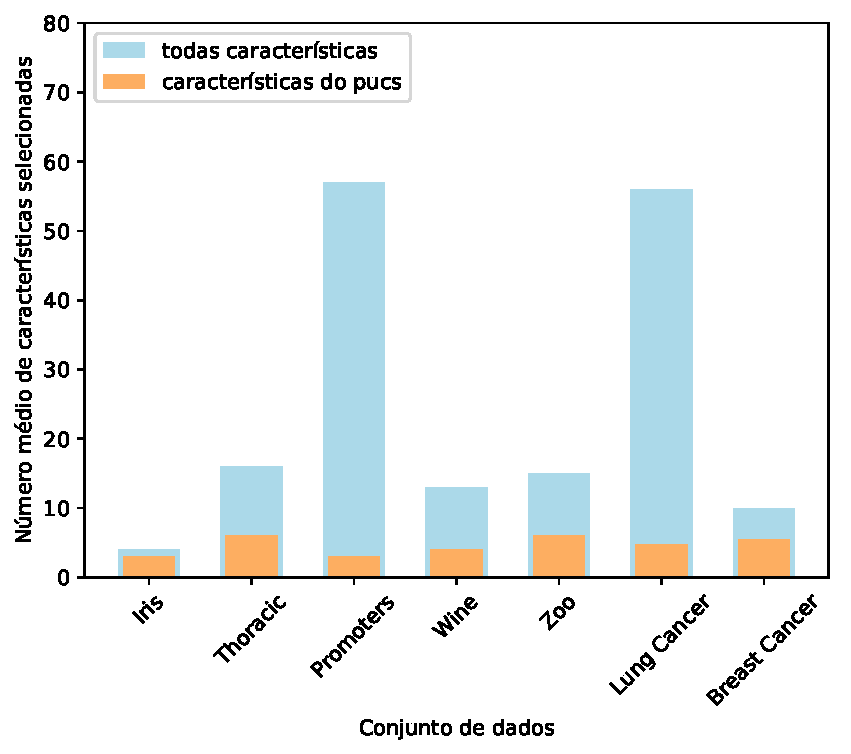
\includegraphics[clip=true, width=0.5\textwidth]{uci/avg_features.pdf}
    }
    &
        \subfigure[] {
        \label{fig:uci:error}
        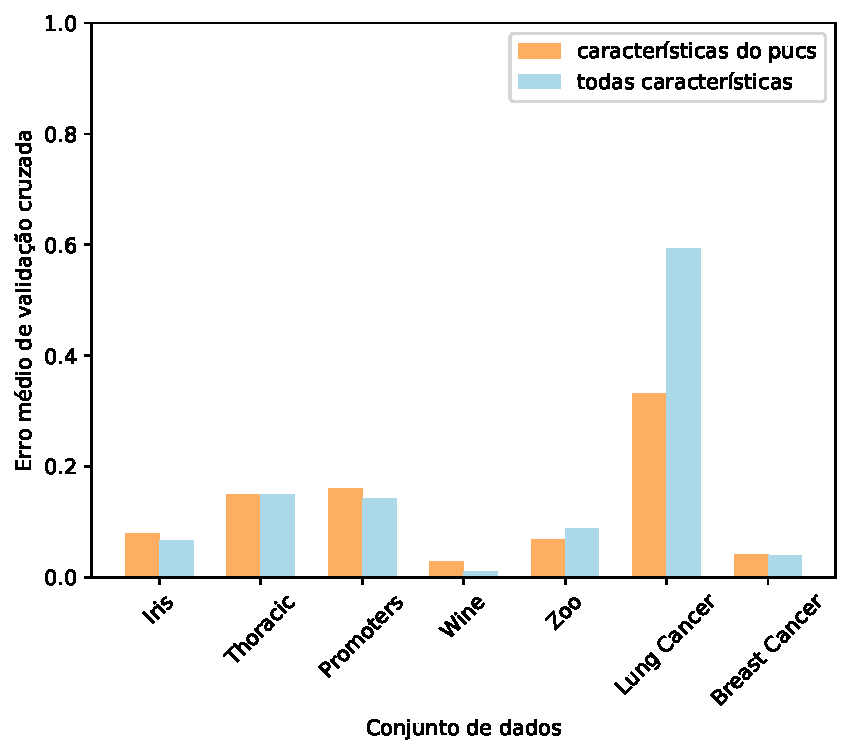
\includegraphics[clip=true, width=0.5\textwidth]{uci/svm_error.pdf}
    }
    \end{tabular}   
    \end{center}
    \caption{Comparações de modelos feitos com todas características e
        com a características selecionadas pelo \algname{PUCS}. A 
        figura~\ref{fig:uci:feats} mostra a quantidade de 
        atributos selecionados pelo algoritmo em cada conjunto
        de dados, enquanto a figura~\ref{fig:uci:error} mostra o erro
        de validação cruzada dos modelos feitos com todas 
        características e apenas com as características selecionadas.}
    \label{fig:uci}
\end{figure}

